\documentclass{article} % For LaTeX2e
\usepackage{nips2015,times}
\usepackage{hyperref}
\usepackage{url}
\usepackage{graphicx}
\graphicspath{ {../assets/} }
\usepackage{biblatex}
\addbibresource{refs.bib}


\usepackage[inline]{enumitem}
\usepackage{booktabs}
\usepackage{multirow}

\title{CSE 546 Assignment 1}


\author{
   Mohammed Nasheed Yasin \\
   Department of Linguistics\\
   University at Buffalo, SUNY\\
   Buffalo, NY 14260 \\
   \texttt{m44@buffalo.edu}
}

% The \author macro works with any number of authors. There are two commands
% used to separate the names and addresses of multiple authors: \And and \AND.
%
% Using \And between authors leaves it to \LaTeX{} to determine where to break
% the lines. Using \AND forces a linebreak at that point. So, if \LaTeX{}
% puts 3 of 4 authors names on the first line, and the last on the second
% line, try using \AND instead of \And before the third author name.

\newcommand{\fix}{\marginpar{FIX}}
\newcommand{\new}{\marginpar{NEW}}

\nipsfinalcopy

\begin{document}


\maketitle

\begin{abstract}
    This report explains our experiments with environments in RL.
    It focuses on the differences between stochastic and deterministic environments,
    and introduces commonly used rendering methodologies. We also go on to solve these
    environments with popular RL tabular methods: Q and Double Q Learning.
\end{abstract}

\section{The Environments}

There are certain features that are common to both the stocastic and deterministic environments.

\subsection*{Environmental Elements}
\begin{figure}[h]
    \begin{center}
        
\includegraphics[width=\textwidth]{elements.png}
    \end{center}
    \label{fig:elements}
    \caption{Environmental elements (from left to right; top to bottom) Agent, Goal,
        Negative Reward, Reward}
\end{figure}

The enivironment is a \verb|6x6| grid. With \verb|36| possible positions that the agent can
occupy. The goal is to reach the oasis (shown in Figure \ref{fig:elements}) \textbf{after
consuming all} the juice (positive reward) within a (configurable) maximum number of time
steps. If the agent lands on a juice tile it is awarded +0.99 and the cactus (negative
reward) leads to a -1.0 reward. Once all the juice is consumed, the agent must proceed to the
oasis to earn a reward of +1.0
The states in this enviroment are a \textbf{combination} of the agent's position and the
current rewards (positive, negative and goal) available on the grid. The Formula \ref{eqn:num-states}
gives us the number of possible states for the agent.

\begin{equation}
    num_{states}=num_{pos} \sum_{k=0}^{c_{reward}} {c_{reward}\choose k}
    \label{eqn:num-states}
\end{equation}

Here $num_{pos}$ refers to the number of grid squares, \verb|36| in our case. $c_{reward}$
refers to the number of positive rewards + the number of negative rewards + 1 (for the goal
state). We have \verb|6| negative rewards, \verb|3| positive rewards and one goal. Hence, 
the $num_{states}$ for us is \verb|36864|.

In each position our agent can take 4 potential actions:
\begin{enumerate*}
    \item Left
    \item Right
    \item Up
    \item Down.
\end{enumerate*}
Resetting the environment will not change the location or distribution of the rewards and
goal state. It only alters the initial state of the agent.

\begin{figure}[h]
    \begin{center}
        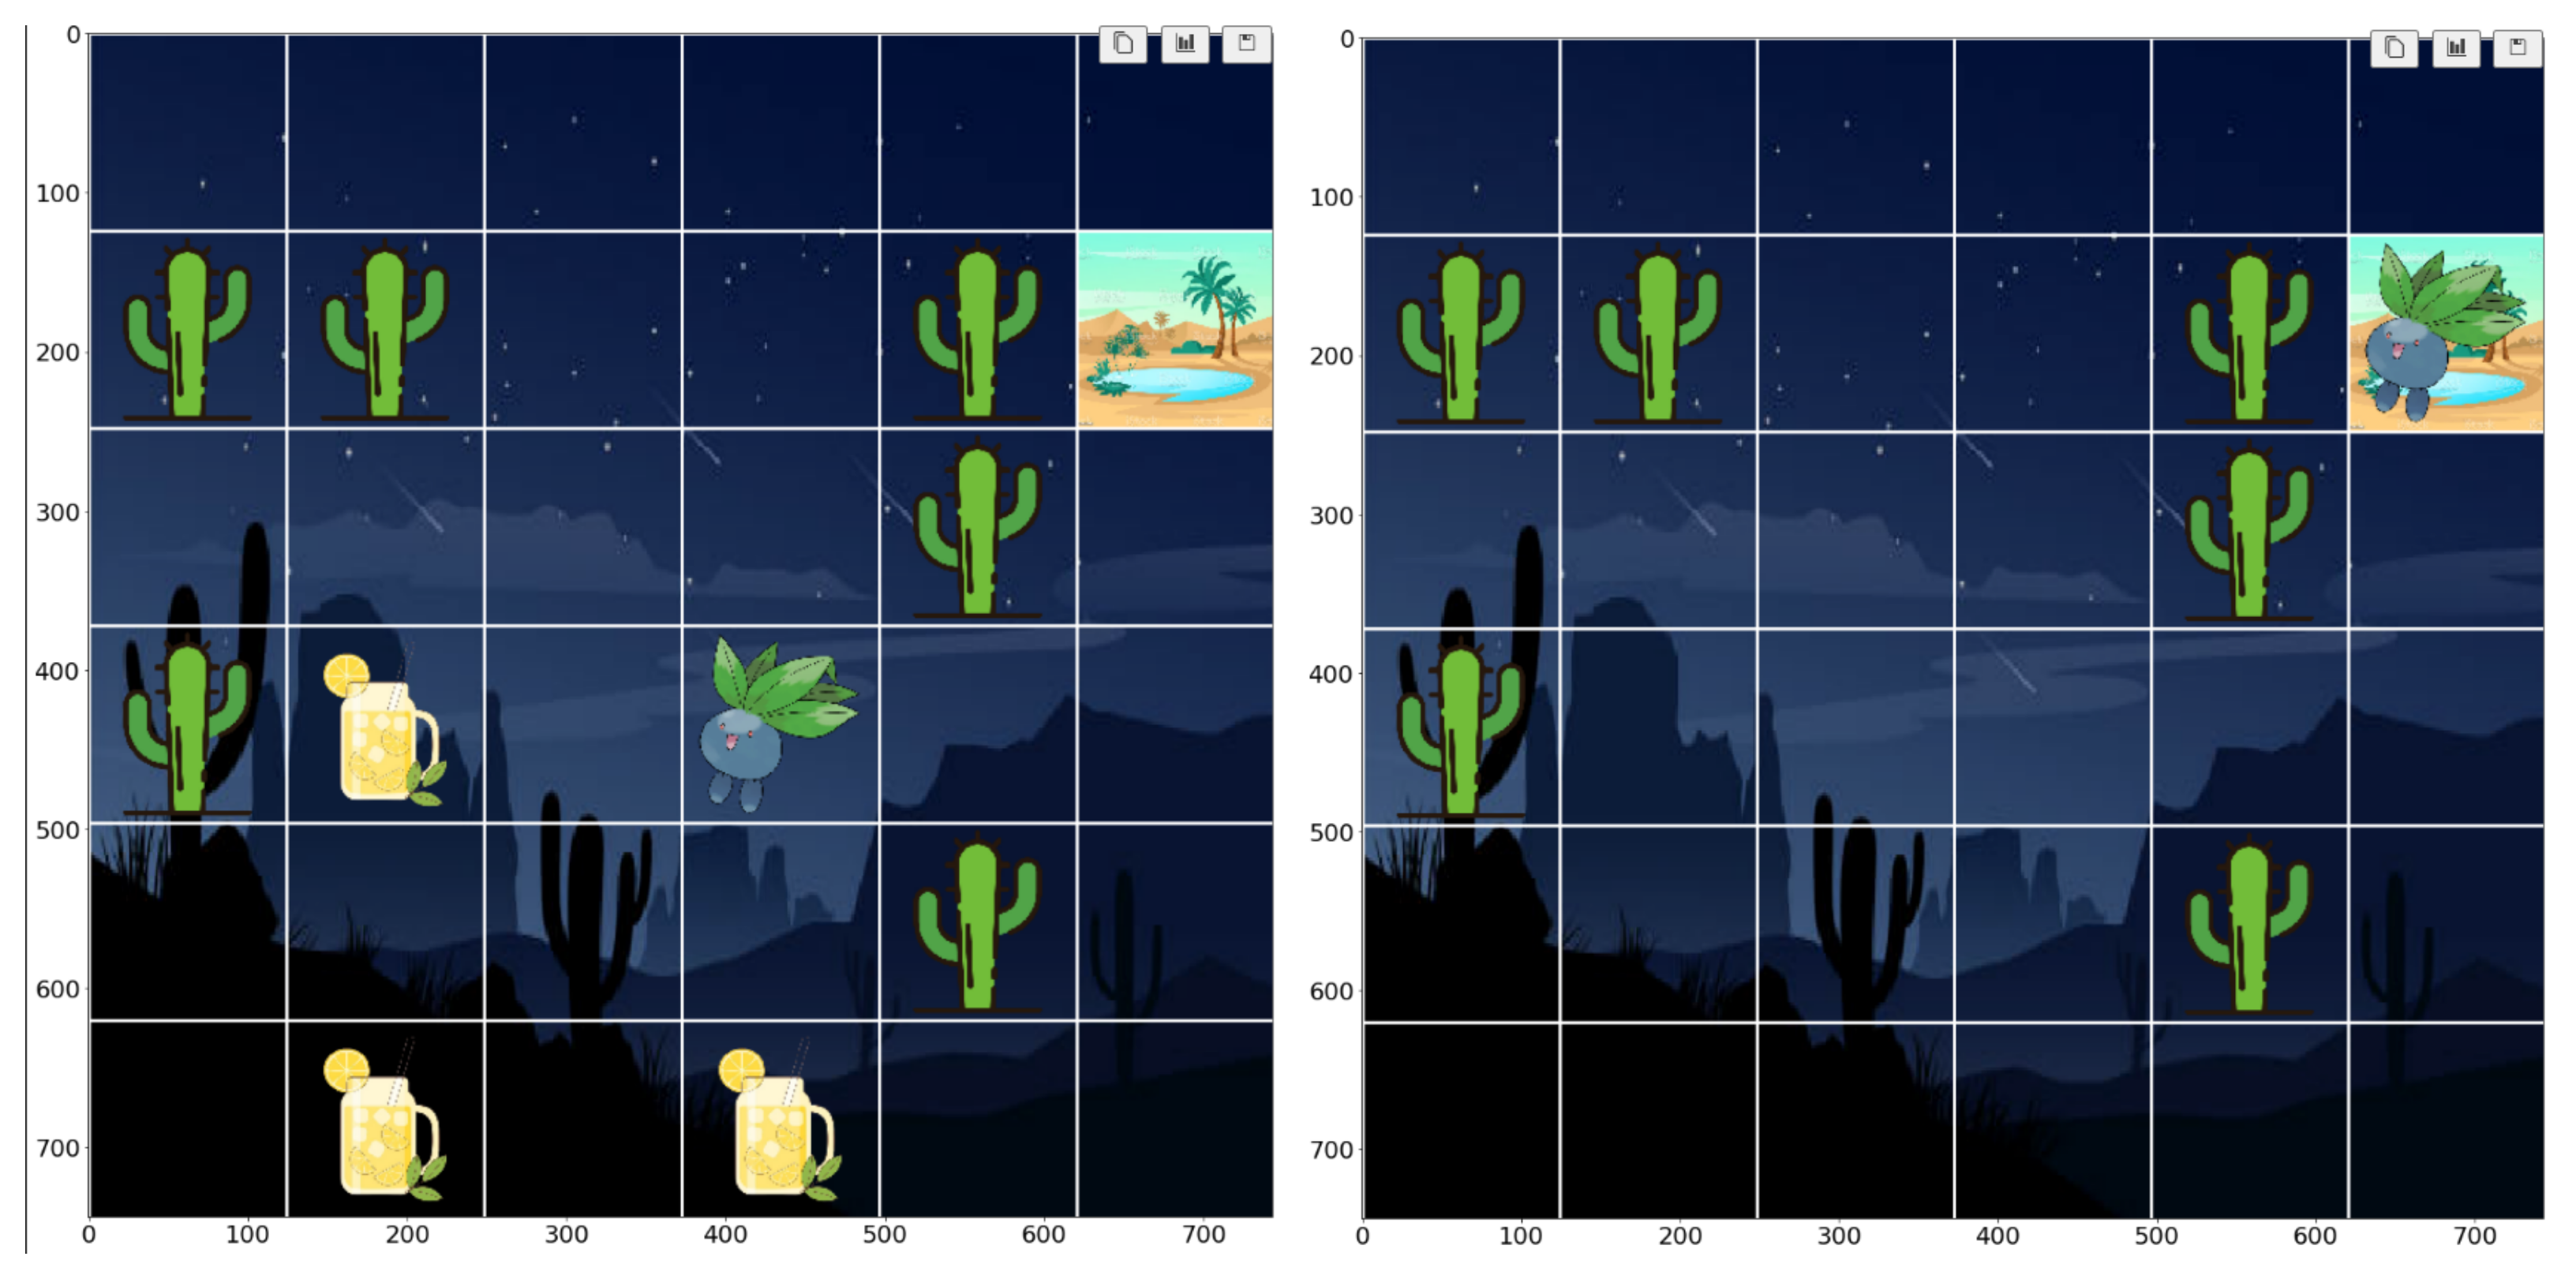
\includegraphics[scale=0.50]{vis.png}
    \end{center}
    \caption{Environment visualizations}
\end{figure}



\subsection{Stocasticity}
An enviroment is called stocastic when the result of an action (i.e. its success or its 
reward) is not guaranteed. Formally, given the same state $s_0$ and action $a$ the next state
$s_1$ and reward $r$ will be probability distributions.

In our \verb|GridEnviroment| the stocasticity can be described as follows:
\begin{itemize}
    \item For every action there is a $2/3^{rd}$ chance that the action is performed as
        expected (\verb|as-is|), a $2/9^{th}$ chance that it is the \verb|double| of what 
        is expected and a $1/9^{th}$ chance of it being a \verb|mirror| action.
    \item A bonus is distributed in a reciprocal proportions. i.e. \verb|0.1x| the
        \verb|max_reward| for coming through the \verb|as-is| action, \verb|0.2x| \verb|max_reward|
        for coming via the \verb|double| action and \verb|0.3x| \verb|max_reward| for the
        \verb|mirror| action.
    \item For instance on a 6x6 grid where the reward on each square is 1 (for simplicity):
    \newline
    If $s_0$ \verb|=(2,3)| and $a$ \verb|= RIGHT|:
        \begin{itemize}
            \item $2/3^{rd}$ chance $s_1$ \verb|=(2,4)| and $r$ \verb|=1+0.1|
            \item $2/9^{th}$ chance $s_1$ \verb|=(2,5)| and $r$ \verb|=1+0.2|
            \item $1/9^{th}$ chance $s_1$ \verb|=(3,2)| and $r$ \verb|=1+0.3|
        \end{itemize}
\end{itemize}

\subsection{Safety in AI}
The following are properties of the environment that ensure valid behavior from the agent:

\begin{enumerate}
    \item We ensure that the agent consumes \textit{all} the \verb|pos_reward| and reaches
        the \verb|goal_state| in the fewest number of steps by imposing a penalty of \verb|0.1x|
        the \verb|max_reward| for every move made.
    \item The reward on all squares is consumed once the agent lands in that state, preventing 
    the agent from settling down in a \textit{high-reward} neighborhood.
    \item The result of any action (left, right, top, down) are clipped to the min and max
        values of 0 and \verb|GridSize| (6 in our case) respectively, ensuring that the
        agent never leaves the environment.
    \item If the agent makes a move but remains in the same spot, we impose the \textit{maximum negative
        reward} (-1.0 in our case). This allows the agent to disincentivize making fruitless
        moves.
    \item We also prevent a \textit{goal rush} (before the agent consumes all the positive
        rewards) by making the goal square unreachable when there are positive reward squares
        left. If the agent takes an action to move into a goal square before collecing all the
        \textit{positive rewards}, they will be kept on the same square, incurring an additional
        penalty (-1.0 in our case) as mentioned in the orevious point.
    \item The stocasticity of the starting point and limited time steps will nudge the agent
        to build strategies that accumulate the maximal reward in the shortest time.
\end{enumerate}

\subsection*{Code Base}
The code for this assignment has been uploaded to \url{https://github.com/nasheedyasin/cse546-rl-assignments}

\begin{figure}[h]
    \begin{center}
        \includegraphics[scale=0.395]{commits.png}
    \end{center}
    \caption{Commit history.}
\end{figure}

\printbibliography

\end{document}